\section{Spezifikation von Einflussfaktoren}
\label{influencingfactors}

Aus denen im Abschnitt \ref{environment} und \ref{futuretrends} dargestellten Umweltfaktoren sowie Zukunftstrends lassen sich nun im Folgenden relevante Einflussfaktoren für den Einsatz von Cloud Computing für die fiktive Skola GmbH herausarbeiten.

\subsection{Ermittlung der Einflussfaktoren}

\FloatBarrier
\begin{table}[!tbp]
	\caption{Übersicht der Einflussfaktor im Suchfeld \textit{Cloud Computing}}
	\begin{center}
		\resizebox{\linewidth}{!}{
			\begin{tabular}{c c c }
				\hline
				\textbf{Nummer} & \textbf{Einflussfaktor} & \textbf{Referenz} \\
				\hline
				1 & Ausfallsicherheit & Gebauer et al. \cite{gebauer }, Schweizer \cite{schweizer} \\
				2 & Informationssicherheit & Gebauer et al. \cite{gebauer}, Meinel et al. \cite{meinel}, \\
				&& Almajalid \cite{almajalid}, Chandra et al. \cite{chandra}, \\
				&& Schweizer \cite{schweizer},  Renz \cite{renz}, \\
				&& Stute \cite{stute} \\
				3 & Störungssicherheit im Netzwerk & Gebauer et al. \cite{gebauer} \\
				4 & Skalierbarkeit & Gebauer et al. \cite{gebauer}, Stieninger \cite{stieninger}, \\
				&& Almajalid \cite{almajalid}, Renz \cite{renz}, Baun \cite{baun} \\
				5 & Flexible Finanzierungsmodelle & Gebauer et al. \cite{gebauer}, Almajalid \cite{almajalid} \\
				6 & Zuverlässige und schnelle & Gebauer et al. \cite{gebauer}, Stieninger \cite{stieninger}, \\
				& Datenübertragung & Almajalid \cite{almajalid}, Baun \cite{baun} \\
				7 & Datenintegrität & Gebauer et al. \cite{gebauer} \\
				8 & Unabhängigkeit vom Anbieter & Gebauer et al. \cite{gebauer}, Grella et al. \cite{grella} \\
				9 & Unabhängigkeit von anderen Nutzern & Gebauer et al. \cite{gebauer}, Grella et al. \cite{grella} \\
				10 & Kontrollmöglichkeiten (on Demand) & Gebauer et al. \cite{gebauer}, Stieninger \cite{stieninger}, \\
				&& Alabbadi \cite{alabbadi} \\
				11 & Reliabilität \& Transparenz & Gebauer et al. \cite{gebauer} \\
				12 & Einhaltung rechtlicher Standards & Gebauer et al. \cite{gebauer}, Stute \cite{stute} \\
				13 & Orts - \& Zeitunabhängigkeit & Stieninger \cite{stieninger}, Meinel et al. \cite{meinel} \cite{meinel2}, \\
				&& Almajalid \cite{almajalid} \\
				14 & Optimierte Ressourcenauslastung & Stieninger \cite{stieninger}, Almajalid \cite{almajalid}, \\
				&& Alabbadi \cite{alabbadi}, Renz \cite{renz} \\
				15 & Energieeffizienz & Stieninger \cite{stieninger} \\
				16 & Modernes Image & Stieninger \cite{stieninger} \\
				17 & Vernetzung von organisatorischen & Stieninger \cite{stieninger}, Meinel et al. \cite{meinel}, \\
				& und prozessualen Strukturen & Chandra et al. \cite{chandra}, Krcmar et al. \cite{krcmar} \\
				18 & Benutzerfreundlichkeit & Stieninger \cite{stieninger}, Almajalid \cite{almajalid} \\
				\hline
			\end{tabular}
		}
		\label{tab:factors1}
	\end{center}
\end{table}
\FloatBarrier

Die Erarbeitung der Einflussfaktoren erfolgte aus einer umfassenden Literaturrecherche sowie Experteninterviews mit Vertretern aus der Bildungsbranche. Innerhalb dieser Literaturrecherche wurde gezielt nach solchen Faktoren gesucht, die verstärkt zu einem Einsatz von Cloud Computing auf Unternehmensebene führten, aber auch nach solchen, die davon abhielten. Dazu gehörten u.a. Ängste und Nachteile der Technologie. Anschließend wurden die gefundenen Faktoren gruppiert und (positive) Einflussfaktoren definiert. Diese finden sich in der Tabelle \ref{tab:factors1}.

Die genauen Beschreibungen aller Einflussfaktoren sind nicht Teil dieser Arbeit. Die große Anzahl an gefundenen Einflussfaktoren stört bei der Erstellung von zukunftstauglichen Szenarien. Nachfolgend sollen diese mittels einem Faktorenportfolio und einer Einflussmatrix weiter eingegrenzt werden.


\subsection{Faktorenportfolio}

Im Folgenden werden aus Gründen der Übersichtlichkeit für die Methoden Faktorenportfolio und Einflussmatrix nur noch die Nummern der einzelnen Einflussfaktoren verwendet. Das Portfolio wird in Abbildung \ref{fig:portfolio} dargestellt und dient zur Ermittlung von kritischen Erfolgsfaktoren. Diese ergeben sich aus der Betrachtungsweise, als dass ihre Bedeutung für einen erfolgreichen Einsatz des Cloud Computing als sehr hoch eingeschätzt wird (Ordinate). Zudem sind eben jene Erfolgsfaktoren derzeit relativ schwach in der Branche etabliert (Abzisse), wodurch sich für die Skola GmbH enorme Potentiale bei der Betrachtung dieser Faktoren ergeben. Die gewählte Methode entfernt somit eher ausgeglichene und überbewertete Einflussfaktoren aus dem weiteren Betrachtungsumfeld.

\begin{figure}
	\centering
	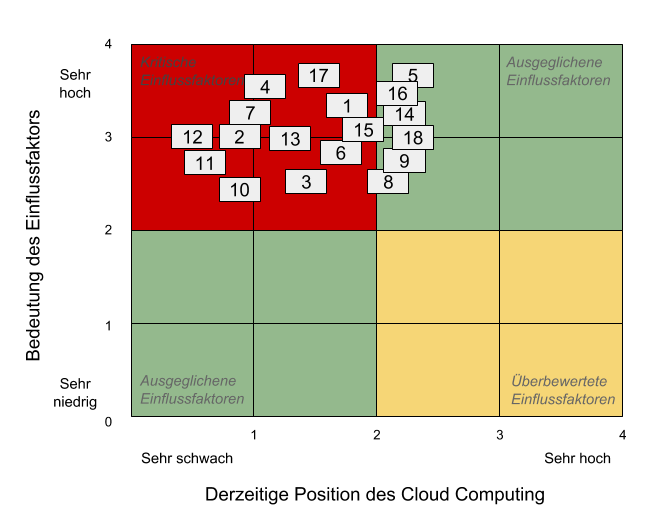
\includegraphics[width=\linewidth]{images/portfolio}
	\caption[Caption for parameters]{Faktorenportfolio}
	\label{fig:portfolio}
\end{figure}

\subsection{Einflussmatrix}

Die in Abbildung \ref{fig:matrix} dargestellte Einflussmatrix soll weiterhin wesentliche Treiber für den erfolgreichen Einsatz von Cloud Computing identifizieren. Eine Wertung von ''0'' kennzeichnet hier einen neutralen Einfluss eines Einflussfaktors auf einen anderen. Mit zunehmender Steigerung der Wertung steigt auch der Einfluss, d.h. eine ''3'' kennzeichnet einen starken Einfluss. 

Die Passivsummen geben eine Übersicht darüber, welche Faktoren stark von anderen beeinflusst werden. Die Faktoren mit einer hohen Passivsumme spielen keine große Rolle in der Gesamtwirkung und werden nachfolgend nicht weiter betrachtet.

Durch die ermittelte Aktivsumme lassen sich Einflussfaktoren erkennen, die im Folgenden näher betrachtet werden sollen. Hierzu werden alle Faktoren eingeschlossen, die eine Aktivsumme von mehr als 10 haben. Dazu gehören ''Informationssicherheit'', ''Störungssicherheit im Netzwerk'', ''Skalierbarkeit'', ''Zuverlässige und schnelle Datenübertragung'', ''Kontrollmöglichkeiten'', ''Orts - \& Zeitunabhängigkeit'' sowie ''Vernetzung von organisatorischen und prozessualen Strukturen''. Besonders das letztgenannte Kriterium fällt durch einen hohen Einfluss im Gesamtkontext hervor. Es lohnt sich somit, diesen Faktor gesondert zu betrachten. Die 7 ermittelten Faktoren mit der höchsten Aktivsumme werden nun als Schlüsselfaktoren identifiziert und nachfolgend genauer beschrieben.

\begin{figure}
	\centering
	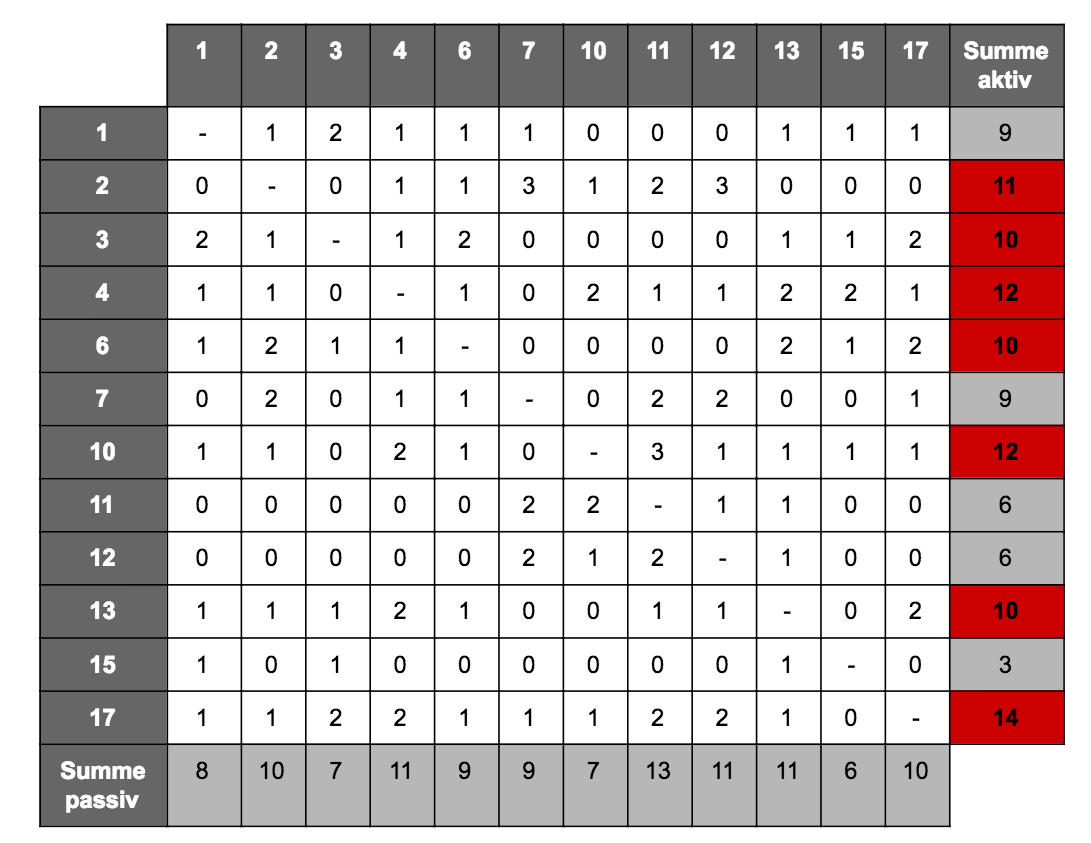
\includegraphics[width=\linewidth]{images/matrix}
	\caption[Caption for parameters]{Einflussmatrix}
	\label{fig:matrix}
\end{figure}

\subsection{Beschreibung der Schlüsselfaktoren}

Nachfolgend sollen die als Schlüsselfaktoren identifizierten Einflussfaktoren genauer beschrieben werden. Als erstes wurde \textit{Informationssicherheit} ermittelt. Innerhalb des Cloud Computing werden Daten zunehmend auf dezentrale Server gespeichert, die nicht mehr direkt im Unternehmen liegen, sondern in externen Rechenzentren \cite{krcmar}. Deshalb obliegt es einer enormen Wichtigkeit, diese Informationen gegen Systemangriffe zu schützen. Nur durch gewisse Sicherheitsvorkehrungen der angebotenen Cloud-Dienste kann ein generelles Vertrauen gegenüber der Technologie entstehen \cite{gebauer}.

Als zweiten Schlüsselfaktor wurde die \textit{Störungssicherheit im Netzwerk} genannt. Cloud Computing kennzeichnet ein hohen Grad an netzwerktechnischen System, gerade wenn ganze Infrastrukturen als Dienstleistung angeboten werden (vgl. IaaS) \cite{krcmar}. Diesbezüglich ist eine gewisse Stabilität des Netzwerkes enorm relevant. Gerade im Umfeld von Schulen, vor allem in ländlichen Regionen, ist eine stabile Netzwerkbandbreite eine generelle Anforderung \cite{gebauer}. Langsame Ladezeiten oder Nichtverfügbarkeit von Materialien durch störanfällige Netzwerke würden zu einer hohen Frustration führen.

Ein großes Schlagwort im Bereich des Cloud Computing ist die \textit{Skalierbarkeit} \cite{renz}. Angebotene Dienste müssen mit den Strukturen des Unternehmens oder mit den Anforderungen im digitalen Lernumfeld mitwachsen. Deshalb ist eine schnelle Anpassbarkeit der angebotenen Dienste auf Kundenwünsche generell sehr wichtig.

Im Kontext des zweiten Faktors (vgl. der Störungssicherheit) steht auch das Kriterium der \textit{zuverlässigen und schnellen Datenübertragung}. Gerade wenn es um die Übertragung von großen Datenmengen geht, ist die Leistungsfähigkeit der der angebotenen Dienste sehr relevant \cite{gebauer}.

Zwar hat der Benutzer durch die Verlagerung in die Cloud weniger Handhabung seine Dienste, jedoch stehen die \textit{Kontrollmöglichkeiten} weiterhin im Vordergrund bei einer erfolgreichen Integration von Cloud Diensten. Hier ist es wichtig, dass der Kunde weiterhin durch flexible Bezahlungmodelle und dynamischen Skalierungsoptionen die Möglichkeit hat, die Dienste nach eigenen Bedürfnissen anzupassen. Dies ist vor allem wichtig im Bezug auf die Lokalisierung der Speicherorte der eigenen Orten, wenn gewisse Datenschutzbestimmungen erfüllt werden müssen \cite{gebauer}.

Gerade im Bezug des mobilen Lernens ist die \textit{Orts - \& Zeitunabhängigkeit} ein sehr wichtiges Kriterium. Der Lernende soll jederzeit und an jedem Ort die Möglichkeit haben, auf Lernmaterialien zugreifen zu können \cite{grella}.

Abschließend stellt die \textit{Vernetzung von organisatorischen und prozessualen Strukturen} einer der wichtigsten Schlüsselfaktoren. Einer der großen Vorteile des Cloud Computing ist die Möglichkeit, viele Dienste über das Internet zu verbinden \cite{krcmar}. Dadurch können enorme Prozessoptimierungen vorgenommen werden, was für die Skola GmbH allein schon aus finanzieller Hinsicht ein wichtiges Indiz wäre.
